%% Created by Yasuyuki SAITO, Department of Information Engineering.


%% 2016/01/13 Edit by Kouta ASAI, and Akira NEMOTO, Advanced Control and Information Engineering Course
%% 2017/12/07 Edit by by Shinichi OEDA, Department of Information Engineering.
%% 「★」マークが変更を加えた部分を表す

%% ★jsarticleに変更 fleqnで数式を左寄せにする
\documentclass[twocolumn, fleqn, uplatex]{jsarticle}

\usepackage{proceeding-DJ}
\usepackage{afterpage}
%% ★数式を使う人が多いと思うので
\usepackage{amsmath}
\usepackage{bm}
\usepackage{booktabs}
\usepackage{enumitem}
\usepackage{makecell}
\usepackage{tabularx}
\usepackage{subcaption}
\usepackage{threeparttable}


%% ★ヒラギノを使っている人向け
\usepackage[deluxe, expert]{otf}

% \makeatletter
% \long\def\@makecaption#1#2{%
%   \vskip\abovecaptionskip
%   \iftdir\sbox\@tempboxa{#1\hskip1zw#2}%
%     \else\sbox\@tempboxa{#1~ #2}%
%   \fi
%   \ifdim \wd\@tempboxa >\hsize
%     \iftdir #1\hskip1zw#2\relax\par
%     \else #1~ #2\relax\par\fi
%   \else
%   \global \@minipagefalse
%   \hbox to\hsize{\hfil\box\@tempboxa\hfil}%
% \fi
% \vskip\belowcaptionskip}
% \makeatother

\begin{document}

\pagestyle{empty}

%% 番号をつけるときはこのすぐ下の行を有効にして,番号を編集する.
%%\date{J--33}
%%所属をDJ以外にしたい場合は,styファイルを編集する.
\date{}
\titleJ{LLMによるプログラミング初学者の\\スキル分析と問題作成による学習支援}
\titleE{LLM-based Skill Analysis and Problem Generation for Learning Support of Novice Programmers}
\authorJ{長谷川 駿一}
\authorE{Shunichi Hasegawa}
\abstract{In programming education for beginners, varying student understanding makes early identification of struggling learners crucial. Prior work used random forest models to classify source code, but struggled with higher-order assessments like problem-solving approaches. This study uses LLMs' NLP capabilities for comprehensive learner assessment and personalized problem generation. Unlike quantitative feature-based methods, we assign LLMs the role of an educator, enabling qualitative source code analysis via prompt engineering techniques like Role-Play Prompting, CoT, Few-Shot Learning, and Self-consistency. Evaluating problems generated by Gemini-1.5-Flush, GPT-4o-mini, and GPT-4o, Gemini excelled in comprehensibility but showed reduced code quality at higher difficulty. GPT-4o-mini showed strengths in engagement and problem quality, potentially boosting motivation. GPT-4o performed consistently well. However, "time appropriateness" was consistently low, highlighting the importance of problem complexity and time limits. These results show LLM-based problem generation can improve learner understanding and motivation, depending on the LLM's characteristics.}
% \keywords{The key word1 of the test for \LaTeXe \ template file, The key
% word2 of the test for \LaTeXe \ template file, The key word3 of the test
% for \LaTeXe \ template file}
\keywords{LLM, Prompt Engineering, Programming Education, Source Code Analysis}
\maketitle

%% 現在ページの上部へのフロートの配置を抑制.
%% ここに記述しておくことで,最初のページの左段上部に図表を置かない.
\suppressfloats[t]


%%●●●●●●●●●●●●●●●
\section{まえがき}
プログラミング初学者の能力判定に関する先行研究として,千枝ら\cite{chieda}は決定木を用いたソースコードの特徴量抽出により学習者の理解度を定量評価する可能性を示唆した.一方,飯棲ら\cite{izumi}はIRMを用いてソースコードの構造的特徴を捉え,より詳細な分析を試みている.先行研究は定量的な学習者理解度把握の可能性を示唆する点で共通するが,特徴量や分析粒度に違いがある.しかし,これらの研究で抽出された特徴量のみでは,学習者の問題解決アプローチといった高次な側面の評価は困難である.

この課題に対し,本研究では,従来の機械学習モデルに代えて大規模言語モデル(LLM)を用いることで,より包括的な学習者評価の実現を目指す.近年,LLMは目覚ましい発展を遂げており,適切なプロンプト設計によってその分析能力を最大限に引き出せることが様々な研究で実証されている\cite{prompting servey}.これらの研究では,k-means法と決定木,そしてIRMといった手法を用いて特徴量抽出が行われているが,本研究では,LLMの持つ自然言語処理能力を最大限に活用し,学習者のスキル分析と個別最適化された問題生成を同時に行うことを目指す.具体的にはプロンプトエンジニアリングの手法を組み合わせることで,LLMに教育者としての役割を与え,学習者のソースコードを分析させ,その分析結果に基づいて個々の学習者に最適な問題を自動生成するシステムの構築を試みる.これは,従来の機械学習アプローチでは困難であった,学習者の問題解決プロセスに対する質的評価と,それに基づく個別最適化された学習支援の実現という,教育工学上の重要課題に対する新たな解決アプローチを提示することを目的とする.

本研究は,プロンプトの最適化を通じて,プログラミング初学者のスキル分析の効率化を図るとともに,分析結果に基づいて学習者の能力に適合した問題を自動生成するシステムの構築を目指しており,LLMを用いた学習者評価の有効性を実証的に示すことで,プログラミング教育におけるLLMの可能性を大きく広げることを目指している.

\section{提案手法}
本研究では,千枝ら\cite{chieda}や飯棲ら\cite{izumi}の研究を推し進め,LLMの高度な自然言語処理能力を活用することで,より包括的な学習者評価と個別最適化された学習支援の実現を目指す.具体的には,LLMに教育者の役割を付与し,ソースコードを直接分析させることで,従来の機械学習アプローチでは困難であった質的な評価を可能にする.

Fig.\ref{fig:system_overview}は,本研究で提案する問題生成システムにおけるプロンプト設計の概要を示している.このシステムは,後述するLLMのプロンプトエンジニアリング手法を統合的に実装している.

\subsection{プロンプトエンジニアリング手法}
このシステムの中核となるのは,LLMの能力を最大限に引き出すためのプロンプトエンジニアリングである.本研究では,以下のプロンプトエンジニアリング手法を組み合わせたアプローチを採用した.
\begin{itemize}
    \item \textbf{Role-Play Prompting}\cite{Role_play}: LLMに教育者としての役割を付与し,学習者評価の専門家としての文脈を確立する.これにより,LLMは教育的な観点からソースコードを分析し,適切なフィードバックや問題生成を行うことが期待される.
    \item \textbf{Chain-of-Thought (CoT)}\cite{CoT}: LLMに段階的な推論を促し,分析プロセスの明示化を行う.これにより,LLMがどのように分析に至ったかの過程を追跡可能にし,結果の妥当性を検証しやすくする.
    \item \textbf{Few-Shot Learning}\cite{Few-shot}: 少数の例題とその分析結果,あるいは問題とその解答例をLLMに提示することで,望ましい出力形式や分析の基準を学習させる.これにより,LLMの出力の質と一貫性を向上させることが期待される.
    \item \textbf{Self-consistency}\cite{Self-consitency}: LLMに複数の問題候補を生成させ,その中から統計的に最も整合性の高い問題を選択するメカニズムを実装する.これにより,LLMの出力の多様性を活用し,より質の高い問題を選択することが可能となる.
\end{itemize}
これらのプロンプト手法を活用した問題生成システムは,以下の3つの段階で構成される.
\begin{enumerate}
    \item \textbf{役割付与とフィードバック指示}\\
    LLMにプログラミング教師としての役割と期待するフィードバックの種類を明示的に伝え,教育的な観点からの分析と問題生成を誘導する.
    \item \textbf{Few-Shot LearningとCoTによる問題生成}\\
    Few-Shot Learningを用いて,過去の学習者の解答例(問題文,ソースコード,模範解答)をLLMに提示し,Chain-of-Thought(CoT)によりソースコードの分析過程とスキル判断の根拠を段階的に出力させる.これにより,学習者の解答傾向や誤りやすい箇所を分析し,適切な問題生成のための基礎情報を獲得する.Few-Shotの例には,学習者のレベルやソースコードの評価情報を含めることで,より適切な問題選定・生成を可能とする.
    \item \textbf{Self-Consistencyによる問題選定と最終出力}\\
    Few-Shot LearningとCoTに基づき生成された複数の問題から,Self-Consistencyの考え方に基づき,同一の入力に対して独立に3つの問題を生成する.その後,再度役割付与とフィードバック指示を行い,LLMに教師としての役割を再認識させた上で,問題の難易度,明確性,独創性などを考慮し,最適な問題を最終出力として選定する.
\end{enumerate}

\begin{figure}
    \centering
    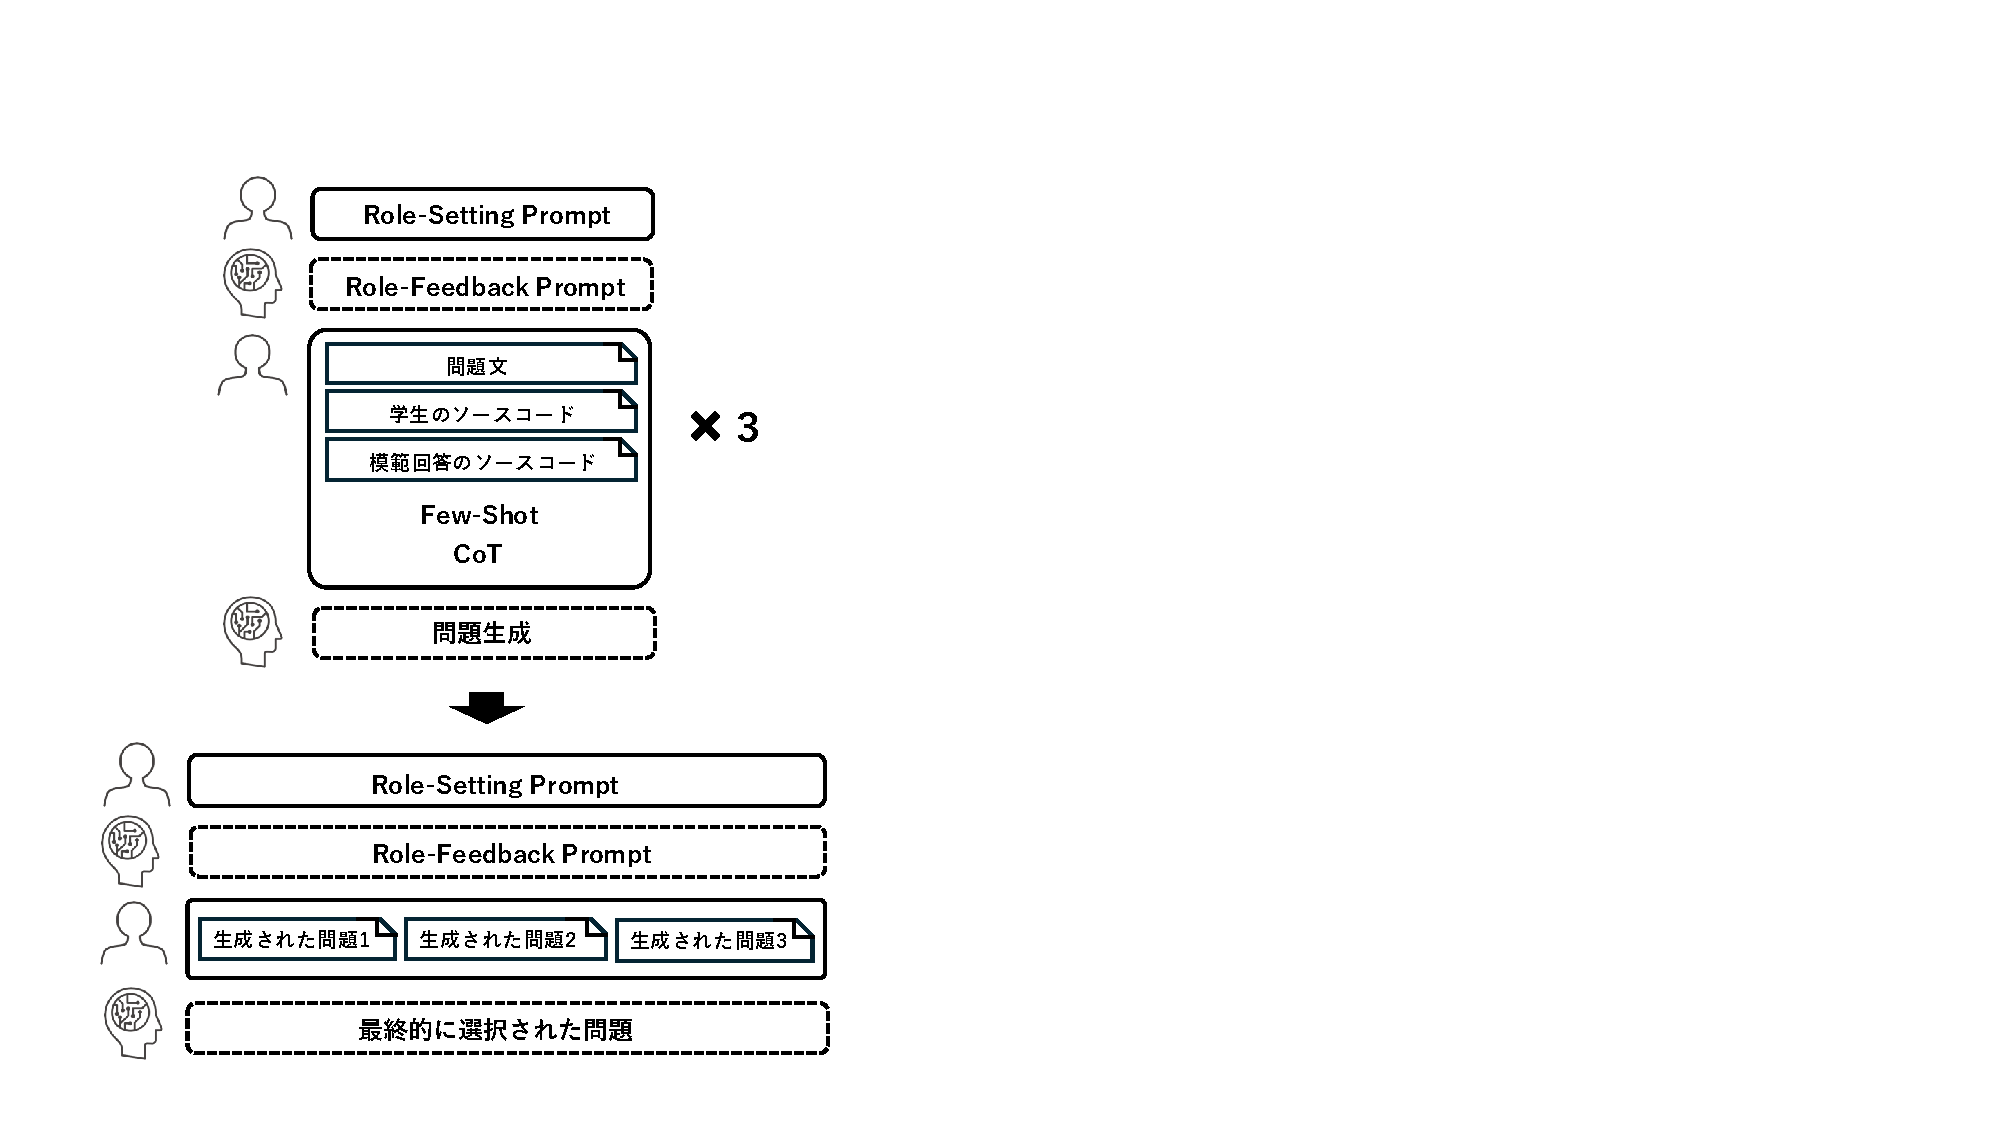
\includegraphics[width=1.0\linewidth]{figure/archtecture_figure_short_tlim.pdf}
    \caption{Overview of the Problem Generation System}
    \label{fig:system_overview}
\end{figure}

\subsection{本研究で使用したLLM}
提案した問題作成システムを実装するLLMの選定は重要な項目の一つである.本研究では性能特性の異なる3種のLLMを比較評価する.Figure.\ref{fig:system_overview}に示す共通のプロンプトを各LLMへの入力として用い,生成された問題を評価することで,各LLMの特性を分析する.以下では,各LLMの概要について述べる.
\begin{itemize}
\item \textbf{Gemini-1.5-Flash} (Google): 大規模なテキストおよびコードベースの文脈理解に優れている.
\item \textbf{GPT-4o-mini} (OpenAI): 比較的軽量な構成ながら,高速な推論処理と多様なタスクへの適応性を特徴とする.
\item \textbf{GPT-4o} (OpenAI): 高度な推論能力とマルチモーダル処理機能を備え,4o-miniと比較してより精緻な自然言語処理が可能である.
\end{itemize}
各LLMの生成した問題の評価は,プログラミング学習者に実際に問題を解答させ,その解答コードとアンケート調査の結果に基づいて行う.本評価では,解答コードの正確性や効率性などを分析するとともに,アンケート調査を通じて被験者の主観的な評価を収集する.


\section{実験概要}
\subsection{実験データ}
本研究では,2024年度木更津工業高等専門学校情報工学科2年の「プログラミング基礎II」後期中間試験の問題と,試験に出席した学生41名が提出したソースコードをデータとして用いた.この試験は筆記試験を含む計7問で構成されており,本研究ではそのうち学生に実際にプログラミングをさせる3問を対象とした.これらの問題文,学生が実際に解いたソースコード,および各問題に対して定義された模範解答のソースコードを用意し,実際の問題生成用プロンプトに組み込んだ.
\subsection{アンケート調査}
Table.\ref{tab:List_Question}は,本実験で使用したアンケート項目を示す.問題生成システムで生成された問題を解いた学生に本アンケートを実施し,問題に対する評価を収集する.


\begin{table}[t]
    \centering
    \caption{List of Questionnaire Items}
    \label{tab:List_Question}
    \footnotesize
    \begin{tabular}{|l|l|}
        \hline
        \textbf{質問項目} & \textbf{評価尺度} \\
        \hline
        \makecell[l]{問題の文章は\\理解しやすかったですか?} & \makecell[l]{10段階評価 \\ (1:わかりにくい,10:わかりやすい)} \\
        \hline
        \makecell[l]{新しいことを学ぶ\\機会になりましたか?} & \makecell[l]{10段階評価 \\ (1:ならない,10:なった)} \\
        \hline
        難易度はどうでしたか? & \makecell[l]{10段階評価 \\ (1:簡単すぎる,10:難しすぎる)} \\
        \hline
        \makecell[l]{この問題を解いて,\\楽しかったですか?} & \makecell[l]{10段階評価 \\ (1:つまらなかった,10:楽しかった)} \\
        \hline
        \makecell[l]{「いい問題だな」\\と思いましたか?} & \makecell[l]{10段階評価 \\ (1:あてはまらない,10:あてはまる)} \\
        \hline
        \makecell[l]{この問題の解答時間である\\15分は適切でしたか?} & \makecell[l]{10段階評価 \\ (1:短かった,10:長かった)} \\
        \hline
    \end{tabular}
\end{table}


\subsection{ソースコードの評価}

\begin{table}[t]
  \centering
  \caption{Evaluation Criteria for Source Code}
  \footnotesize
  \label{tab:List_Source}
  \begin{tabular}{|l|l|} % 説明部分の幅を指定
    \hline
    \textbf{評価項目} & \textbf{説明} \\
    \hline
    正確性 & \makecell[l]{問題を解決できているかを評価.} \\
    \hline
    効率性 & \makecell[l]{アルゴリズムの選択や実装の最適性を評価.} \\
    \hline
    可読性 & \makecell[l]{コードの読みやすさ,命名規則の適切さ,\\構造の整理などを評価. }\\
    \hline
    基礎概念 & \makecell[l]{コードが適切なプログラミング概念を\\適切に活用しているかを評価.} \\
    \hline
  \end{tabular}
\end{table}

本研究では,Table.\ref{tab:List_Source}の評価項目を用いて,GPT-4oによる自動コード評価を行った.各項目は5段階で評価し,5点を最高評価,1点を最低評価とした.5段階評価を採用したのは,評価の粒度と評価のしやすさのバランスを考慮したためである.

\section{実験結果}
\subsection{各モデルのアンケート回答傾向}

Table.\ref{tab:mean_values}に各モデルのアンケート回答の平均値を示す.Gemini-1.5-Flushは「理解しやすさ」で最も高い平均値 $(M=7.40)$ を示し,問題の一貫性を示唆する結果となった.GPT-4o-miniは「楽しさ」 $(M=6.55)$ と「良問評価」 $(M=6.63)$ で若干高い評価を得ており,学習意欲を高める問題生成に強みを持つ可能性が示唆された.GPT-4oは全体的に中間的な評価を示し,バランスの取れた問題生成を行う傾向が見られた.全モデルで「時間の適切さ」の評価が比較的低く $(M=4.34\sim4.56)$,設定時間(15分)が短すぎた可能性が示唆された.また,ソースコード評価は全モデルで低い傾向が見られ,コード品質の改善の余地が示された.

\begin{table}[t]
\centering
\footnotesize
\caption{Average Scores of Survey Items for Each Model}
\label{tab:mean_values}
\begin{tabular}{lccc}
\toprule
アンケート項目 & Gemini-1.5-Flush & GPT-4o & GPT-4o-mini \\
\midrule
理解しやすさ & 7.40 & 6.97 & 6.00 \\
新しい学び & 5.69 & 5.89 & 5.37 \\
難易度 & 5.51 & 5.75 & 4.92 \\
楽しさ & 6.51 & 6.03 & 6.55 \\
良問評価 & 6.43 & 6.22 & 6.63 \\
時間の適切さ & 4.49 & 4.56 & 4.34 \\
\bottomrule
\end{tabular}
\end{table}

\subsection{モデル比較(一元配置分散分析とTukeyのHSD検定)}

各モデルの評価を比較するため,アンケート調査の各指標に対して一元配置分散分析とTukeyのHSD検定を実施した.Table.\ref{tab:anova_results}に示すように,「理解しやすさ」において統計的に有意な差 $(F=3.0928, p=0.0495)$ が確認された.TukeyのHSD検定(Table.\ref{tab:tukey_hsd_understanding})の結果,Gemini-1.5-FlushとGPT-4o-mini間に有意差 $(p=0.0456)$ が認められ,Gemini-1.5-Flushが生成する問題が最も理解しやすいことが示された.他のアンケート指標では有意な差は見られなかった.

\begin{table}[t]
\centering
\footnotesize
\caption{Results of One-Way ANOVA on Survey Data}
\label{tab:anova_results}
\begin{tabular}{lccc}
\hline
評価項目 & $F$値 & $p$値 & 有意性(5\%水準) \\
\hline
理解しやすさ & 3.0928 & 0.0495 & 有意差あり \\
新しい学び & 0.3899 & 0.6781 & 有意差なし \\
難易度 & 1.5028 & 0.2272 & 有意差なし \\
楽しさ & 0.5317 & 0.5891 & 有意差なし \\
良問評価 & 0.2966 & 0.7440 & 有意差なし \\
時間の適切さ & 0.1000 & 0.9049 & 有意差なし \\
\hline
\end{tabular}
\end{table}

\begin{table}[t]
\centering
\scriptsize
\caption{Results of Tukey's HSD Test for "Ease of Understanding}
\label{tab:tukey_hsd_understanding}
\begin{tabular}{lccccc}
\hline
比較 & 平均差 & $p$値  & 有意性(5\%水準) \\
\hline
GPT-4o vs. GPT-4o-mini & -0.9722 & 0.2142  & 有意差なし \\
GPT-4o vs. Gemini-1.5-Flush & 0.4278 & 0.7474  & 有意差なし \\
GPT-4o-mini vs. Gemini-1.5-Flush & 1.4 & 0.0456 & 有意差あり \\
\hline
\end{tabular}
\end{table}

\subsection{各指標との相関分析}

各モデルにおけるアンケート調査指標とソースコード評価指標間の相関分析を行った結果(Table.\ref{tab:correlation_results_focused}),特にGemini-1.5-Flushにおいて顕著な傾向が認められた.「難易度」とソースコードの各評価指標(正確性,効率性,可読性,基本概念)の間には強い負の相関 $(r=−0.657\sim−0.759)$ が観察され,難易度が高いと判断された問題ほどコード品質が低下する傾向が示された.また,「時間の適切さ」とソースコードの各評価指標の間には中程度の正の相関 $(r=0.444\sim0.614)$ が見られ,問題に取り組む時間が適切であると感じるほどコード品質が向上する傾向が示唆された.さらに,「新しい学び」とソースコードの各評価指標の間には中程度の負の相関 $(r=−0.417\sim−0.566)$ が見られ,新しい学びが多いと感じるほどコード品質が低下する傾向が示された.これは,新しい概念学習時にコードの完成度よりも学習に重点が置かれるためと考えられる.他のモデルでは,Gemini-1.5-Flushで見られたような顕著な相関は見られなかった.

\begin{table}[t]
\centering
\scriptsize
\caption{Correlation of key elements}
\label{tab:correlation_results_focused}
\begin{threeparttable}
\begin{tabular}{lccc}
\hline
評価指標の比較 & Gemini-1.5-Flush & GPT-4o & GPT-4o-mini \\
\hline
難易度 vs. 正確性 & \textbf{-0.738} & \textbf{-0.559} & \textbf{-0.328} \\
難易度 vs. 効率性 & \textbf{-0.693} & \textbf{-0.377} & \textbf{-0.488} \\
難易度 vs. 可読性 & \textbf{-0.657} & \textbf{-0.447} & \textbf{-0.468} \\
難易度 vs. 基本概念 & \textbf{-0.759} & \textbf{-0.428} & \textbf{-0.488} \\
\hline
時間の適切さ vs. 正確性 & \textbf{0.614} & 0.327 & 0.213 \\
時間の適切さ vs. 効率性 & \textbf{0.600} & 0.246 & 0.241 \\
時間の適切さ vs. 可読性 & \textbf{0.444} & 0.308 & 0.236 \\
時間の適切さ vs. 基本概念 & \textbf{0.609} & \textbf{0.421} & 0.210 \\
\hline
新しい学び vs. 正確性 & \textbf{-0.566} & -0.131 & -0.224 \\
新しい学び vs. 効率性 & \textbf{-0.417} & -0.188 & -0.254 \\
新しい学び vs. 可読性 & \textbf{-0.511} & -0.206 & -0.263 \\
新しい学び vs. 基本概念 & \textbf{-0.485} & -0.274 & \textbf{-0.312} \\
\hline
\end{tabular}
\begin{tablenotes}
\small
\item 注:相関係数の絶対値が0.4以上を中程度以上の相関として太字で示している.
\end{tablenotes}
\end{threeparttable}
\end{table}
\section{考察}
Gemini-1.5-Flushは,生成する問題の理解しやすさという点では優れているものの,難易度が上がるとコード品質が低下する傾向が見られた.この結果は,問題の難易度調整と生成されるコードの品質維持を両立させることの難しさを示唆している.一方,GPT-4o-miniは,学習者の動機づけを高めるような問題作成に強みを持つ可能性が示された.これは,問題の提示方法を工夫することで学習意欲を効果的に高められることを示している.また,GPT-4oは各評価項目において安定した性能を示しており,多様な学習ニーズに対応できる可能性を示唆している.しかしながら,全モデルを通して時間配分が課題として浮上しており,問題の複雑さと制限時間との関係性を適切にモデリングする必要性が明らかになった

\section{まとめ}
本研究は3種類のLLMを用いて個々の学習者に合わせたプログラミング問題生成を試み、学習支援への応用可能性を探った。実験でLLMは可能性を示したものの、教育的視点に基づく問題設計が不可欠と示唆された。今後の課題は、難易度調整、時間配分、フィードバック提供といった教育要素へのLLM活用を検討すること。今後の研究では、問題の多様性拡大(アルゴリズム、データ構造等)、コード自動評価、学習履歴との連動、各LLMの特性を活かした問題生成方法確立を目指し、より効果的な学習支援システム開発を目指す。

\subsection*{謝辞}
本研究はJSPS 科研費 19H01728 の助成を受けたものです.

\begin{thebibliography}{9}
  \renewcommand{\baselinestretch}{1.0}
  \bibitem{chieda}千枝睦実, 大枝真一,“プログラミング授業での決定木を用いたドロップアウト原因の可視化,” 2019 年情報科学技術フォーラム, 2019.
  \bibitem{izumi}飯棲俊介, 大枝真一,“IRM(Infinite Relational Model)と決定木を用いたプログラミ ング初学者の能力判定のための特徴量の抽出,”IEICE Conferences Archives.
  \bibitem{prompting servey}Schulhoff, Sander, et al."The Prompt Report: A Systematic Survey of Prompting Techniques." arXiv preprint arXiv:2406.06608 (2024).
  \bibitem{Role_play}Kong, Aobo, et al."Better zero-shot reasoning with role-play prompting." arXiv preprint arXiv:2308.07702 (2023).
  \bibitem{CoT}Suzgun, Mirac, et al. "Challenging big-bench tasks and whether chain-of- thought can solve them." arXiv preprint arXiv:2210.09261 (2022).
  \bibitem{Few-shot}Brown, Tom, et al. "Language models are few-shot learners." Advances in neural information processing systems 33 (2020): 1877-1901.
  \bibitem{Self-consitency} Wang, Xuezhi, et al. "Self-consistency improves chain of thought reasoning in language models." arXiv preprint arXiv:2203.11171 (2022).

  
\end{thebibliography}

\end{document}
